\documentclass{article}
\usepackage[utf8]{inputenc}
\usepackage[spanish]{babel}
\usepackage{amsthm}
\usepackage{amsmath}
\usepackage{amssymb}
\usepackage{graphicx}
\usepackage{wrapfig}
\usepackage[letterpaper, top=0.78in, bottom=0.78in, left=0.98in, right=0.98in]{geometry}
\usepackage[hidelinks]{hyperref}
\usepackage{url}
\usepackage{soul}

\decimalpoint
\renewcommand{\baselinestretch}{1.5}

\begin{document}
    \begin{titlepage}
        \begin{center}
            % School logo
            \begin{figure}
                \centering
                
\includegraphics[scale=0.13]{/home/mona/Pictures/logo_itesm.png}\\ % Logo de la institución
            \end{figure}
            \vspace{5cm}
            % School data
            \LARGE{Instituto Tecnológico y de Estudios Superiores de Monterrey}\\
            \vspace{1cm}
            \large Escuela de Ingeniería y Ciencias \\
            \vspace{0.2cm}
            \large Ingeniería en Ciencias de Datos y Matemáticas \\
            \vspace{0.2cm}
            \large Uso de álgebras modernas para seguridad y criptografía \\
            \vspace{1cm}
            \textbf{Implementación de criptografía de clave pública para protección de comunicaciones con IoT en entornos de monitoreo y consumo de energía.}\\ % Nombre de la tarea
            \vspace{0.7cm}
            % Tabla de integrantes del equipo
            \begin{table}[h!]
                \centering
                \begin{tabular}{ ||c|c|| }
                    \hline
                    Nombre & Matrícula \\
                    \hline
                    Juan Pablo Echeagaray González & A00830646 \\
                    \hline
                    Ricardo Camacho Castillo & A01654132 \\
                    \hline
                    Michelle Yareni Morales Ramón & A01552627 \\
                    \hline
                    Emily Rebeca Méndez Cruz & A00830768 \\
                    \hline
                    Daniela García Coindreau & A00830236 \\
                    \hline
                    Carolina Longoria Lozano & A01721279 \\
                    \hline
                \end{tabular}
            \end{table}
            \vspace{0.7cm}
            \large 	Dr. Alberto F. Martínez \\ % Nombre del profesor 1
            \vspace{0.2cm}
            \large 	Dr. Daniel Otero Fadul\\ % Nombre del profesor 2
            \vspace{0.2cm}
            \large Socio Formador: COCOA, LICORE \\
            \vspace{0.2cm}
            \large Monterrey, Nuevo León \\
            \vspace{0.2cm}
            \large 17 de marzo del 2023 \\
            \vspace{1cm}
        \end{center}
    \end{titlepage}
    % \maketitle

    \tableofcontents
    \listoffigures
    \listoftables
    \clearpage
    \renewcommand{\tablename}{Tabla}

    \section{Introducción}

        \subsection{Situación en México}

            En el 2015, se estableció una ley llamada "Ley de transición energética." El objetivo de esta ley es regular el uso de la energía sustentable, así como la obligaciones en materia de energías limpias y reducción de emisiones de contaminantes en la industria eléctrica. Para así mantener la competitividad de los sectores productivos. \cite{gobmx} En otras palabras, esta ley busca tener un incremento gradual de la participación de la energías limpias en la industria eléctrica con el objetivo de reducir emisiones.

            Hoy en día, existen muchos países que están trabajando en esta transición para poder llegar al 100\% de uso de energía renovable. Como se observa en la Figura \ref{fig:energiaM} Brasil es el país con el porcentaje más alto de uso de energía renovable arriba del 80\%, seguido por Canadá con el porcentaje de uso arriba del 60\%, seguido por Alemania, Inglaterra, Italia y Turquía con un porcentaje arriba del 40\%. En la gráfica se observa que México esta posicionado en decimoquinto lugar con un porcentaje aproximadamente del 20\% y además se observa que entre los años 2015 y 2020, México tuvo un incremento de uso de energía renovable del 31\%. \cite{climate_transparency}

            \begin{figure}[h]
                \centering
                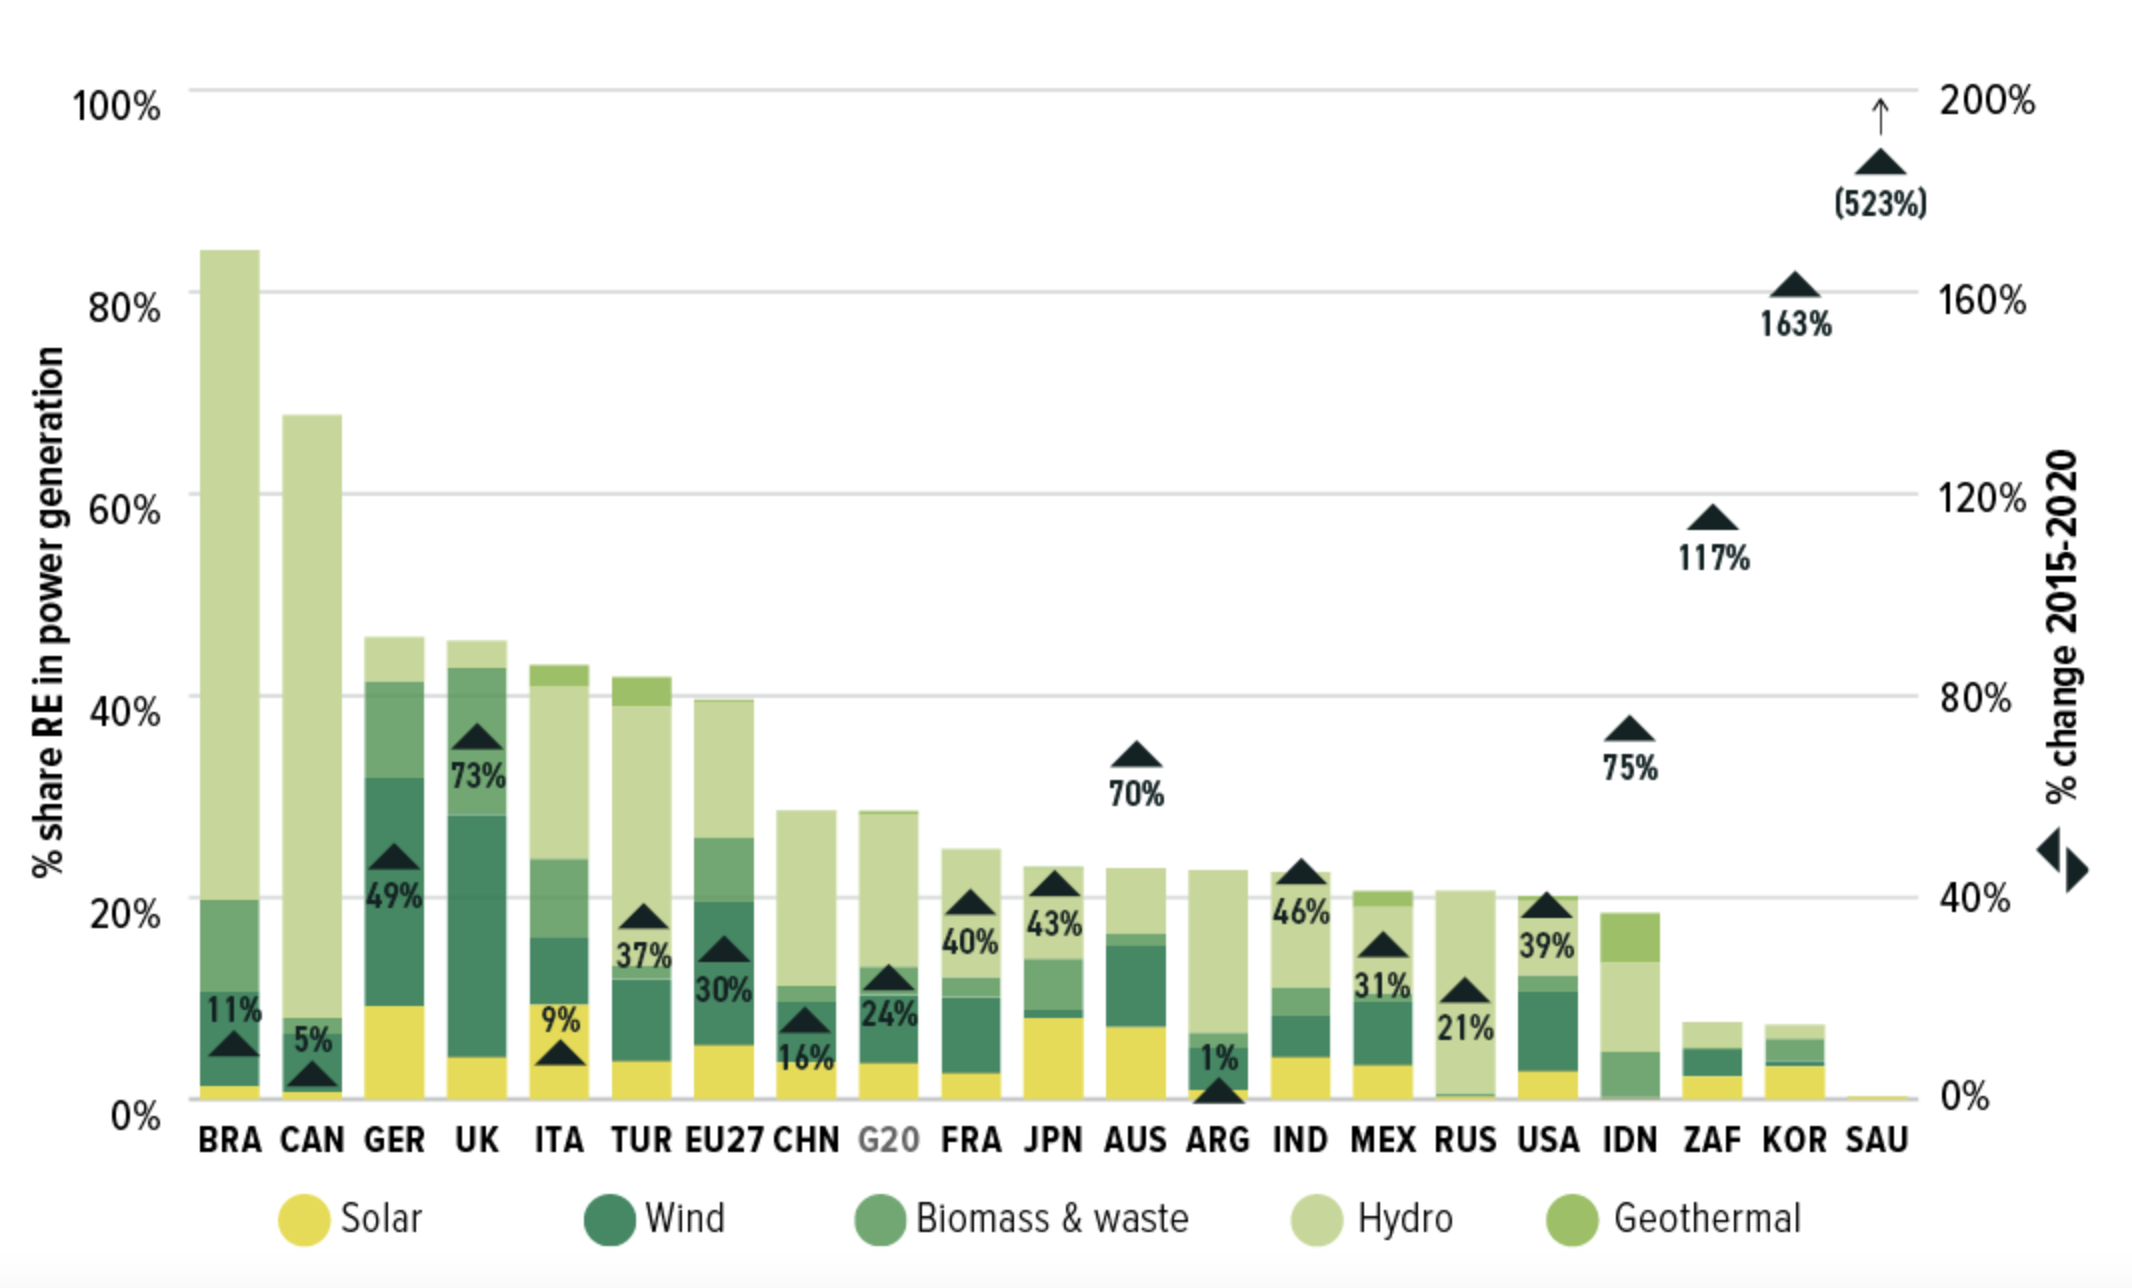
\includegraphics[scale = 0.30]{img/energiaMundo.png}
                \caption{Porcentaje de uso de energía renovable por país en el 2021 \cite{climate_transparency}}
                \label{fig:energiaM}
            \end{figure}

            Actualmente, México cuenta con un combinación de varios tipos de energía renovable: solar, eólica, hidroeléctrica, geotérmica, nuclear e instalaciones de bioenergía. México es el segundo país en América Latina con el sector de energía solar más grande, con una capacidad instalada un poco más de 7 GW en 2021, seguido por la energía eólica en 7.7 GW, luego la producción geotérmica con 976 MW. \cite{mexico} Hoy en día, se cuenta con 300,624 instalaciones y se espera que para el 2023 se tengan más de 500 mil instalaciones.

            Sin embargo, aunque el sector de energía renovable siga creciendo desde su primera operación en el 2007 con su primer planta, muchas de estas instalaciones solamente se instalan y se olvidan no los consultan ni dan seguimiento a mantenimiento. Por esta razón, se busca mejorar la situación de la red de situación para que sea más inteligente y contar con medidores inteligentes que ayuden a saber que esta sucediendo con la instalación.

        \subsection{Sobre el reto}

            El entorno de comunicación actual requiere la protección de datos durante el tránsito y el almacenamiento. En el caso concreto del trabajo que se está realizando, el objetivo es imaginar e implementar importantes proyectos criptográficos públicos en entornos IoT. En otras palabras:

            \begin{itemize}
                \item Los esquemas de clave pública deberán funcionar en ambientes con recursos restringidos.
                \item La comunicación entre todos los elementos involucrados deberá ser segura.
                \item Los esquemas de clave pública deberán involucrar el uso de esquemas lightweight.
                \item Los datos almacenados en el centro de control deberán estar encriptados
                \item Deberá existir un canal de comunicación bidireccional entre el centro de control y los auditores.
            \end{itemize}

            \begin{figure}[h]
                \centering
                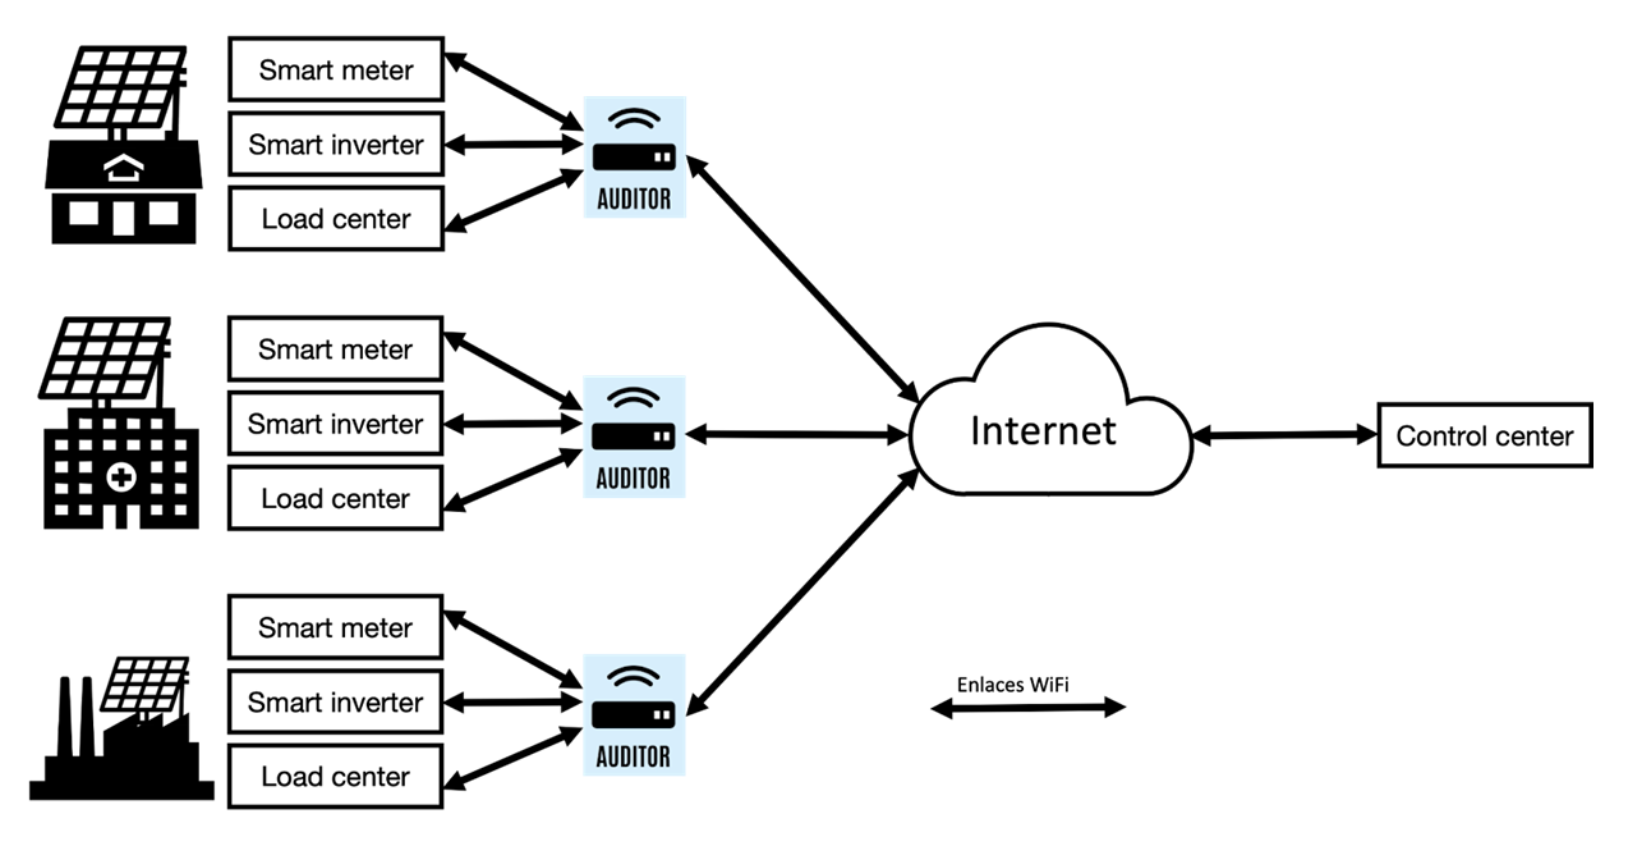
\includegraphics[scale = 0.30]{img/dataExchange.png}
                \caption{Intercambio de Datos a ser Protegido}
                \label{fig:dataExchange}
            \end{figure}

            Para fines de este reto, como podemos ver en la Figura \ref{fig:dataExchange}, en primera instancia, se busca proteger el intercambio de información entre el auditor y el control center. Algunas características que se desean proveer son:
             \begin{itemize}
                \item \textbf{Confidencialidad:} Se busca que solamente los elementos involucrados accedan a la información proporcionada por los sensores. Se aplica la misma condición cuando se almacenan los datos en el Centro de Control, para que puedan revisar dicha información todos los que estén autorizados a hacerlo.
                 \item \textbf{Integridad:} Se busca que la información provista por los sensores no sea alterada y se pueda verificar dicha condición. Lo mismo aplica cuando dicha información se almacene en el Centro de Control.
                 \item \textbf{Autenticidad:} Se desea que cada sensor pueda ser monitoreado e identificado, para así determinar qué datos generaron.
             \end{itemize}

             Además, de la Figura \ref{fig:dataExchange} podemos observar los siguientes componentes:

             \begin{itemize}
                 \item Dispositivos smart que serán los encargados de monitorear parámetros de energía cada cierto tiempo (smart meter, smart inverter, load center). Estos dispositivos contarán con una interfaz WiFi para comunicarse con el exterior. Para fines del reto, los datos comunicados por estos dispositivos serán proporcionados por la OSF “en crudo” para que puedan ser utilizados. Se manejarán de forma muy cautelosa los datos.
                 \item Auditores digitales que recolectarán datos de los dispositivos smart conectados a ellos. Para fines del reto, consideren:
                 \begin{enumerate}
                     \item El uso de tarjetas Arduino o Raspberry con capacidad WiFi.
                     \item Usar sus equipos de cómputo para habilitarlos como auditores, pero considerando que la solución debe ser consistente como si estuvieran usando una Raspberry o un Arduino.
                 \end{enumerate}
                 \item El control center que será capaz de consultar el estado previo y actual de cada dispositivo smart  conectado a los auditores.
             \end{itemize}

            En este reto se estará trabajando con la organización socio-formadora COCOA Collabrorative Innovation B.V. COCOA es una organización impulsada por la innovación con el uso de la tecnología digital. Su enfoque principal es la innovación digital para abordar desafíos de la sostenibilidad actual. Específicamente, trabajan con monitoreo de datos para la sostenibilidad, herramientas de apoyo a la toma de decisiones espaciales y finanzas sostenibles/climáticas. Además, la organización busca aportar eficiencia y transparencia a los esfuerzo globales para el logro de los Objetivos de Desarrollo Sostenible (ODS). \cite{cocoa} Actualmente, ellos trabajan con la empresa LICORE, una organización mexicana que se centra en el desarrollo de tecnología electrónica para la industria de la eficiencia energética y las redes inteligentes.

            La organización socio-formadora propone el siguiente escenario para el reto como se observa en la Figura \ref{fig:esquema} Se tendrán dos auditores, un auditor reporta datos de un medidor inteligente y el otro auditor reporta datos de un inversor inteligente. Los datos de los auditores serán proporcionados por el socio-formador. Los datos que se estarán recolectando de estos dispositivos tendrán que viajar por el internet protegidos hasta que lleguen al centro de control. En el centro de control, los datos serán almacenados en una base de datos en donde tendrán que ser almacenados de manera encriptada.

             \begin{figure}[h]
                \centering
                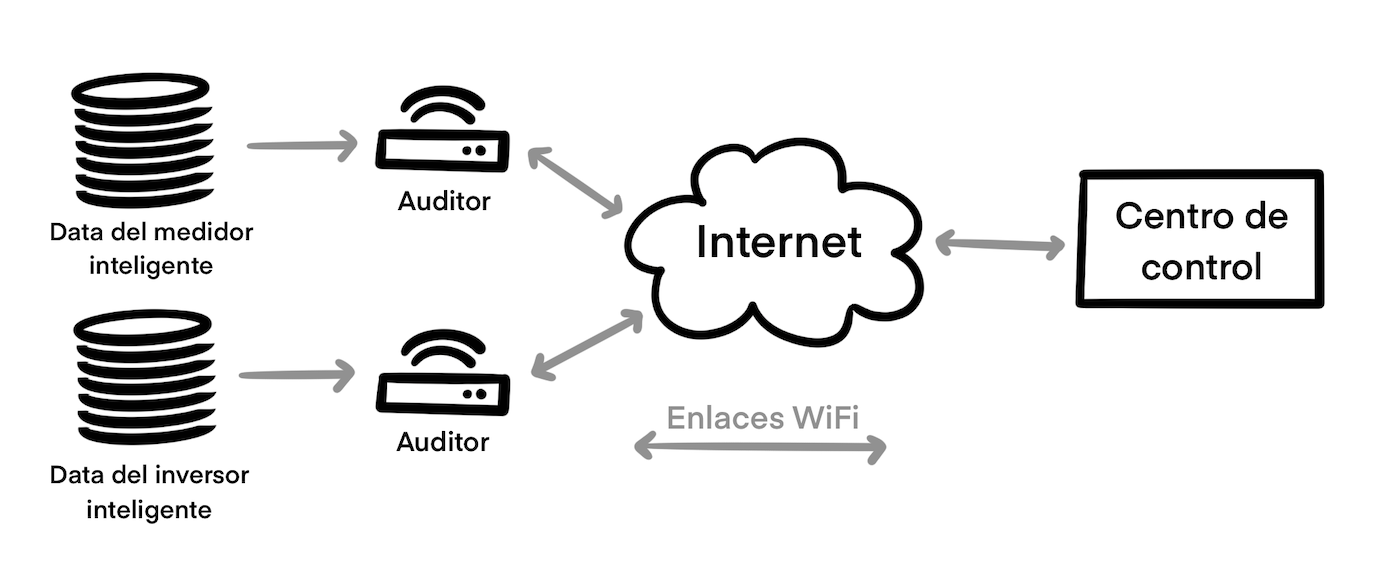
\includegraphics[scale=0.35]{img/esquema_reto.png}\\
                \caption{Esquema sugerido para la prueba de concepto (PdC).}
                \label{fig:esquema}
            \end{figure}

            En general, el objetivo principal del reto es implementar protocolos de criptografía de clave pública para proteger el intercambio de datos de sensores en ambientes IoT, los datos que se estarán manejando son datos que tienen que ver con el monitoreo y consumo de energía, estos datos sensibles. Los protocolos se buscan aplicar de manera balanceada. Además, se busca que el intercambio de datos sea de manera automática ya que los datos tienen que ver con el estados de los sensores en un dicho tiempo al igual que la actualización de su firmware.

    \section{Estado del Arte} \label{sec:introduction}

        En el artículo 'Internet of things: Privacy issues revisited' menciona que el anonimato en la comunicación tiene el objetivo de proteger los datos de tráfico para que la información se mantenga confidencial, pero incluso si el contenido de la comunicación se mantiene confidencial puede llegar a filtrarse por datos de tráfico que incluyen identidades y ubicaciones de las partes que se están comunicando, hora, frecuencia y volumen de la comunicación \cite{Weber}.

        A continuación se presentarán algunos estudios y trabajos relacionados al análisis de los sistemas IoT:

        De acuerdo al artículo 'Métodos de criptografía ligera para brindar servicios de seguridad al Internet de las Cosas' dentro de los nodos del IoT se encuentran restricciones como bajo poder computacional, alimentación por baterías o se presenta un ancho de banda limitado. Dentro del artículo se buscan métodos novedosos para servicios de seguridad por medio de la criptografía ligera, estos métodos permitirán garantizar la seguridad de la información para estos sistemas restringidos \cite{criptografia_ligera}.
        Por el momento no existe una definición precisa en el estado del arte para el término algoritmo 'ligero', pero se emplea para referirse a diseños arquitecturales simplificados que reducen el número de operaciones que ejecuta con un impacto moderado dentro de la seguridad del algoritmo.

        Los autores definen la criptografía ligera como '\textit{la rama de la criptografía que estudia el uso de algoritmos criptográficos adaptados a los requerimientos de aplicaciones que cuentan con recursos limitados en materia de: capacidad de procesamiento, hardware disponible, memoria, energía, canal de comunicaciones, entre otros}' \cite{criptografia_ligera}.
        En el escrito se propone como solución, en el caso de hardware, la implementación de sistemas de seguridad e introducir aceleradores de cómputo, en el caso de software, el uso  de un coprocesador como un circuito integrado de aplicación especifica.

        En el artículo 'Aseguramiento de dispositivos IoT con Blockchain e Infraestructura de Clave Publica' se demuestra el poder de unir diferentes tecnologías, el blockchain y la clave publica, para conseguir acceso remoto confiable. Utilizan el uso de computación distribuida, bases de datos de-centralizadas y distribuidas, algoritmos criptográficos y blockchain híbridas. Por medio de una metodología de auditoría de riesgos, evalúan dos dispositivos en su estado natural y los cambios que tienen al implementarse la clave publica distribuida por blockchain. En ambos dispositivos el riesgo final fue menor al riesgo inicial, probando la eficacia del método.

        Según el Ing. Omar Paniagua en su artículo \cite{villagomezdiseno} mencionó sobre el diseño de un prototipo IoT para pruebas de penetración y monitoreo de la seguridad en un sistema de domótica. Un sistema de domótica es el conjunto de maquinas con cierto nivel de inteligencia artificial que permite la automatización y que realice acciones dependiendo de los fenómenos captados por los elementos electrónicos interconectados. El prototipo de domótica se desarrolló para hacer pruebas de ataque y monitorear el comportamiento del sistema de detección y prevención de intrusos (IDS/IPS) en el sistema de domótica, el prototipo detectó satisfactoriamente los escaneos y pruebas de ataque, sin embargo, ante un ataque DDoS (denegación de servicio distribuido desde varios hosts) pueden llegar a denegar el servicio al sistema. \cite{villagomezdiseno}  En general, en el artículo concluyó que las medidas clave que garantizan una mayor seguridad son las siguientes:
        \begin{itemize}
            \item Autenticar todas las entidades del IoT que se pueden unir a la red de domótica utilizando criptografía de clave pública y certificados X.509 firmados por una autoridad raíz de confianza. Estos deben almacenarse siguiendo estándares de procesamiento FIPS. \cite{villagomezdiseno}
            \item Para la seguridad del hardware se deben implementar protocolos de cifrado como TLS/DTLS para una transferencia segura, la integridad de datos se debe basar en hashes criptográficos SHA, se deben usar firmas digitales para el intercambio de datos, los datos deben clasificarse según la seguridad a niveles y datos críticos y esquemas de AAA/CIA, todo el software y firmware tiene que ser verificado, los sistemas informáticos deben mantenerse actualizados con parches de seguridad y toda la infraestructura centralizada debe de ser protegida contra la denegación de servicio por ataques DDoS. \cite{villagomezdiseno}
        \end{itemize}

    \subsection{Arquitecturas de intercambio de información}

        \subsubsection{P2P}

            La OSF es trabaja con un tipo de arquitectura de intercambio de información denominada peer-to-peer, que es una red de dispositivos de cómputo en donde todos o algunos aspectos funcionan sin clientes ni servidores fijos, ya que se trata de una serie de nodos que actúan simultáneamente como clientes y servidores respecto a otros nodos. De esta manera los usuarios pueden colocar archivos para compartir y todos los demás usuarios de la red pueden acceder a él.

            Este tipo de redes permiten el intercambio de información en cualquier formato entre los ordenadores interconectados y una de las principales características de estos programas es que permiten visualizar el tráfico y controlar la velocidad de descarga de los archivos. Además, puede existir comunicación en tiempo real ya que cuentan con sistema de chat. \cite{p2p}

        \ul{Tipos de redes P2P}

        \begin{enumerate}
        \item \textbf{Redes centralizadas:} son aquellas que trabajan con un sólo servidor que aloja toda la información
        \item \textbf{Redes híbridas:} trabajan con varios servidores centrales y las descargas se ejecutan de los nodos.
        \item \textbf{Redes descentralizadas:} trabajan con el sistema de nodos de modo que no utilizan servidores centrales de ningún tipo.%\cite{p2p.2}
        \end{enumerate}

        \ul{Ventajas y desventajas}

        La ventaja de este tipo de redes es que permite compartir archivos de manera sencilla sin necesitar un servidor central, sin embargo, existen algunas desventajas ya que los nodos no son identificables y esto podría derivarse en fraude, virus o contenido ilícito, además, si los nodos dejan de aportar recursos no conseguirán la información deseada.


    \subsection{Recursos disponibles}
    Los recursos que se necesitarán para dar solución al reto son los siguientes.
    \begin{itemize}
        \item  Datos recolectados por los dispositivos Smart, que serán proporcionados por la OSF.
        \item Auditores digitales, que implican también el uso de otros recursos.
        \begin{itemize}
            \item Tarjetas Arduino o Raspberry con capacidad Wifi.
            \item Equipos de cómputo para habilitarlos como auditores
        \end{itemize}
    \end{itemize}
%\cite{p2p.3}
    \subsection{Arranque de la red}






        \subsection{Side Channel Attacks}

            Una dimensión más a considerar en el diseño e implementación de un protocolo criptográfico es la susceptibilidad del sistema a ser víctima de \textit{Ataques de Canal Lateral} (Side Channel Attacks). Este tipo de ataques se enfoca en la extracción de información latente generada por dispositivos pequeños que implementan algoritmos criptográficos \cite{shim2015survey}.

            Un atacante que busque vulnerar dichos dispositivos físicos puede realizar análisis de:
            \begin{itemize}
                \item Consumo energético
                \item Tiempo de cómputo
                \item Radiación electromagnética
            \end{itemize}

            Para mitigar el posible daño ocasionado de estos ataques se proponen 2 líneas de acción; modificaciones a la implementación del algoritmo criptográfico a nivel software, y adecuaciones en el hardware del dispositivo. Las modificaciones de software incluyen ruido aleatorio dentro de las señales, cambiar de forma aleatoria el orden en que se realizan los comandos (cuando aplique), añadir instrucciones falsas. A nivel de hardware las modificaciones se enfocan en enmascarar el consumo energético del dispositivo mediante la generación de ruido, o la aleatorización del cómputo (clock).

            %- El dispositivo se tiene que conectar a internet por medio de cable ethernet? O es desde Wifi que se conecta al internet?
            %- El sensor recibe su fuente de energía de la generada por el panel solar? O es independiente?
            %- Parece ser que una opción viable para este reto es el uso de curvas elípticas, en clase se mencionó que ofrecen el mismo nivel de seguridad que otros algoritmos, pero con muchos menos requerimientos de espacio y poder computacional
            %	- Analizar nuitka, pypi, cython para compilar el código fuente que generemos, debería de aumentar la velocidad base del algoritmo, y reduce el tamaño
            %- Considerar vulnerabilidades "side channel attack" una vez que hayamos implementado el algoritmo criptográfico

    \section{Propuesta de solución del reto} \label{sec:introduction}



    \subsection{Blockchain}
     Blockchain es una forma nueva de documentar datos que consiste en una serie de datos inmutables, compartibles y con marca de tiempo los cuales son administrados por un grupo de computadoras.

    La información de blockchain, también llamada "cadena de bloques", se distribuye por medio de libros de contabilidad, libros los cuales registran la información en una comunidad. Cada transacción de cada uno de estos bloques debe de ser validada por cada uno de los miembros, además, existe una copia de dicha información para todos los involucrados, por lo que alterar los datos anteriores es imposible gracias al consenso. \cite{blockchain_education} \\

    Estos libros de contabilidad sirven como una herramienta que determina la propiedad de cierto activo en cualquier momento, independientemente del tipo que tenga. La información de la cadena de bloques puede ir desde transferencias de dinero, documentos de identidad, propiedades, o cualquier otra información que requiera la validación de ambas partes para la confirmación y la responsabilidad. \cite{blockchain_tec} \\

    Blockchain para empresas usa un registro compartido e inmutable al que sólo tienen acceso los miembros que tienen permiso. Los miembros de dicha red puede controlar qué información es visible para cada miembro u organización, así como también las acciones que pueden tomar.

    Blockchain ofrece beneficios comerciales como el ahorro de costos debido a una mayor eficiencia, velocidad y automatización. Blockchain reduce en gran medida el papeleo y los errores, se reducen los costos generales y de transacciones, para así reducir o eliminar la necesidad de que intermediarios o terceros tengan que verificar las transacciones.

    Tipos de Blockchain:
    \begin{enumerate}
        \item \textbf{Blockchains Públicas:} Cualquiera puede descargar, adaptar o personalizar y realizar transacciones. Este tipo de blockchain requiere millones de máquinas. Produce la mayor inmutabilidad y transparencia, sin embargo, también tiene la máxima ineficiencia ya que los costos de almacenamiento y de electricidad que tiene son muy altos, además de la baja velocidad de transacción.
        \item \textbf{Blockchains privadas:} Funcionan sólo por invitación y siguen un conjunto de reglas creadas por los que invitan. Debido a que hay un bajo número de personas que están involucradas, puede que sea más especializado, con altibajos con menor inmutabilidad y transparencia, una mayor centralización, eficiencia, velocidad y volumen de transacción. De esta manera se reduce el costo y los recursos utilizados.
        \item \textbf{Consorcios blockchain:} Este tipo de blockchain es un híbrido entre lo probado y lo público, también funciona sólo por invitación o por solicitud, pero todas las personas invitadas tienen los mismos derechos de voto cuando toman decisiones por consenso.
    \end{enumerate}

    Ventajas de la tecnología Blockchain
    \begin{itemize}
        \item \textbf{Autenticidad:} Los usuarios tienen la posibilidad de mantener privados todos sus datos personales y de almacenamiento al mismo tiempo que pueden identificarse.
        \item \textbf{Confianza:} Brinda suficiente confianza a las personas en las operaciones par poder llevar a cabo transacciones como certificados o pagos.
        \item \textbf{Transparencia y origen:} Los usuarios pueden realizar transacciones teniendo el conocimiento de que cada una de las partes puede participar en la transacción.
        \item \textbf{Inmutable:} Los registros son escritos y almacenados de forma permanente sin ninguna modificación, esto los vuelve inmutables.
        \item \textbf{Descentralizada:} La nece-sidad de una autoridad centralizada que este a cargo de las transacciones y el mantenimiento de registros es eliminada.
        \item \textbf{No hay mediadores:} Es posible que los usuarios realicen transacciones directamente entre ellos sin la necesidad de una tercera persona que funja de mediador.
    \end{itemize}
        \clearpage
        \bibliographystyle{IEEEtran}
        \bibliography{references.bib}

\end{document}

% /home/mona/Pictures/logo_itesm.png